\documentclass[12pt]{report}
\usepackage[utf8]{inputenc}
\usepackage[T1]{fontenc}
\usepackage[french]{babel}
\usepackage{graphicx}
\usepackage{hyperref}
\usepackage{lmodern}
\usepackage{fancyhdr}
\usepackage{geometry}
\usepackage{float}


\geometry{margin=2.5cm}
\pagestyle{fancy}
\fancyhf{}
\rhead{\thepage}
\lhead{
\includegraphics[width=1.8cm]{Logo_nanterre.png}} % logo école en en-tête

% PAGE DE GARDE CUSTOM
\begin{document}

\begin{titlepage}
    \centering
    
\includegraphics[width=3.5cm]{Logo_nanterre.png}\par\vspace{1cm}
    {\scshape\LARGE Université Paris Nanterre\par}
    \vspace{0.5cm}
    {\huge\bfseries Rapport de Projet\par}
    \vspace{0.5cm}
    {\Huge\bfseries AutoPredict\par}
    \vspace{1.5cm}
    {\Large \textbf{Membres du projet :} \par}
    \vspace{0.3cm}
    {\Large X. Frédéric \\ R. Yann \\ R. Jérémy \par}
    \vfill
    {\large \today\par}
\end{titlepage}

\tableofcontents

\chapter{Présentation de AutoPredict}
\section{Problématique}
Le choix d’une voiture peut s’avérer complexe pour un acheteur, en particulier lorsque de nombreux critères entrent en jeu : budget, type de motorisation, consommation, puissance, style, marque, etc. Les plateformes existantes n’offrent pas toujours une expérience personnalisée ou intuitive pour explorer l’offre de véhicules selon ses préférences réelles. Par ailleurs, les vendeurs ou les analystes souhaitent mieux comprendre les facteurs qui influencent le prix d’un véhicule, et optimiser leur stratégie de vente.


\section{Solution}
AutoPredict est une plateforme web intelligente permettant d’exploiter une base de données automobile pour proposer deux fonctionnalités principales :

\begin{itemize}
    \item \textbf{Recherche assistée de modèles} : à partir d’un budget donné et de certaines préférences (ex. type de transmission, puissance, taille...), l’utilisateur reçoit une liste de véhicules correspondant à ses besoins.
    \item \textbf{Estimation de prix} : à partir des caractéristiques sélectionnées (ex. année, style, consommation...), l’utilisateur obtient une estimation de la fourchette de prix des véhicules correspondants.
\end{itemize}

Ces fonctionnalités sont rendues possibles grâce à une architecture combinant analyse de données, machine learning, backend intelligent et une interface frontend intuitive.

\section{Public cible}

Notre projet AutoPredict s’adresse à deux types d’utilisateurs principaux, chacun ayant des besoins distincts que nous avons pris en compte dans la conception de notre moteur de recommandation et dans la structuration de notre analyse.

\subsubsection{Vendeurs de véhicules particuliers}

Les vendeurs, qu’il s’agisse de particuliers ou de petites structures de revente, cherchent à positionner correctement leurs modèles sur le marché. AutoPredict les aide à :
\begin{itemize}
    \item fixer un prix de vente cohérent et compétitif en fonction des caractéristiques techniques du véhicule (année, style, puissance, segment de marché) 
    \item anticiper la valeur de revente selon la dépréciation attendue, pour optimiser leurs marges 
    \item identifier les catégories ou styles de véhicules les plus demandés selon les tendances observées
\end{itemize}

\subsubsection{Acheteurs de véhicules d’occasion ou neufs}

Les acheteurs utilisent AutoPredict comme outil d’aide à la décision pour affiner leur recherche selon leurs préférences et contraintes personnelles. Notre outil leur permet :
\begin{itemize}
    \item de filtrer les véhicules selon des critères personnalisés (budget, consommation, motorisation, marque, popularité) 
    \item de découvrir des modèles correspondant à leur profil d’usage (familial, urbain, plaisir, économique) 
    \item d’évaluer si un modèle est bien positionné en termes de rapport qualité/prix, à partir des données du marché
\end{itemize}
Nous explorerons en détail les spécificités de chaque groupe cible, à travers nos personas.

\section{Personas utilisateurs}

Afin de mieux illustrer les usages concrets de notre plateforme AutoPredict, nous avons défini deux \textit{personas} représentant les profils types de nos utilisateurs cibles : un vendeur de véhicule et un acheteur. Ces profils permettent de centrer notre réflexion sur leurs attentes spécifiques et d’adapter les fonctionnalités de notre outil à leurs besoins.

\subsubsection{Persona 1 : Julien, vendeur de voitures d’occasion}
\begin{figure}[H]
\centering
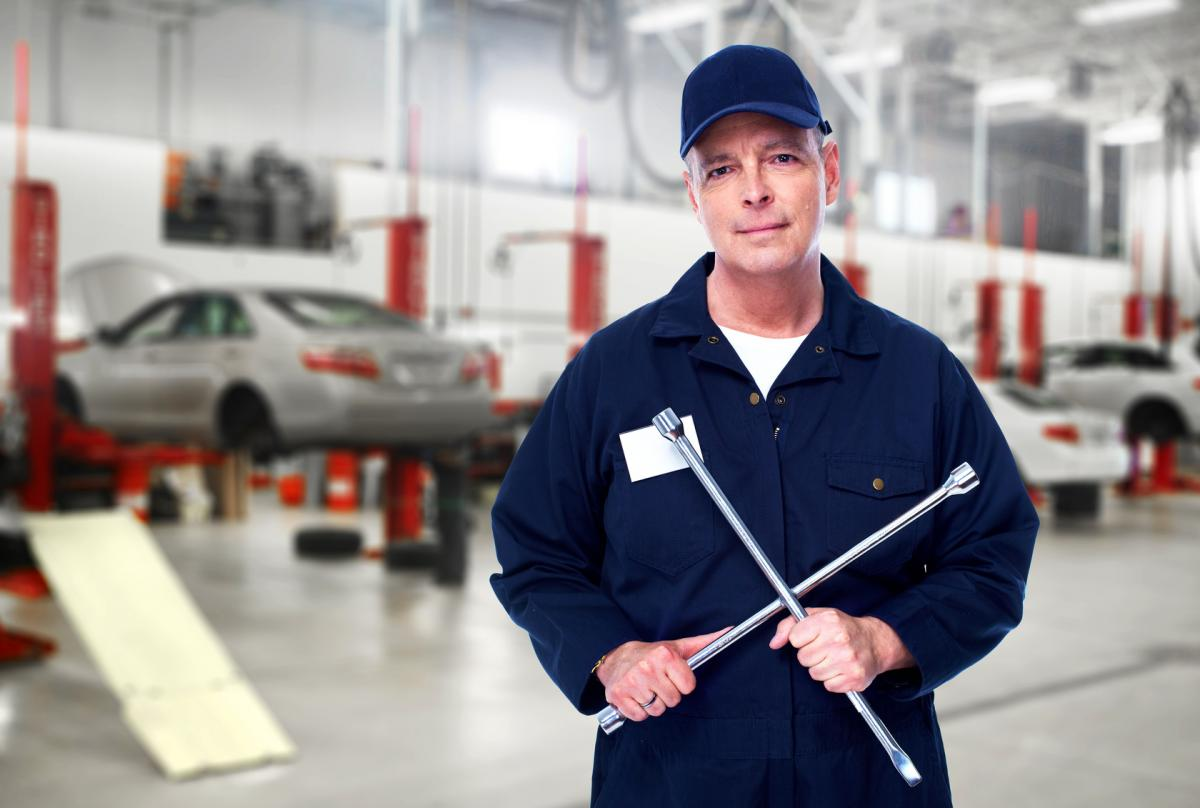
\includegraphics[width=0.5\textwidth]{Julien.jpg}
\end{figure}

\begin{itemize}
    \item \textbf{Âge} : 42 ans
    \item \textbf{Profession} : Garagiste indépendant
    \item \textbf{Localisation} : Angers
    \item \textbf{Objectif} : Vendre ses véhicules au bon prix en s’alignant sur les tendances du marché
    \item \textbf{Comportement} :
    \begin{itemize}
        \item Dispose d’un stock varié de véhicules d’occasion
        \item Cherche à évaluer la valeur de chaque voiture en fonction de ses caractéristiques (année, style, puissance, consommation...)
    \end{itemize}
    \item \textbf{Besoins couverts par AutoPredict} :
    \begin{itemize}
        \item Obtenir une estimation juste du prix de vente d’un modèle spécifique
        \item Identifier les caractéristiques qui influencent le plus la valeur résiduelle d’un véhicule
        \item Visualiser les tendances de consommation, de prix ou de popularité par segment de marché
    \end{itemize}
\end{itemize}

\subsubsection{Persona 2 : Clara, acheteuse de voiture citadine}

\begin{figure}[H]
\centering
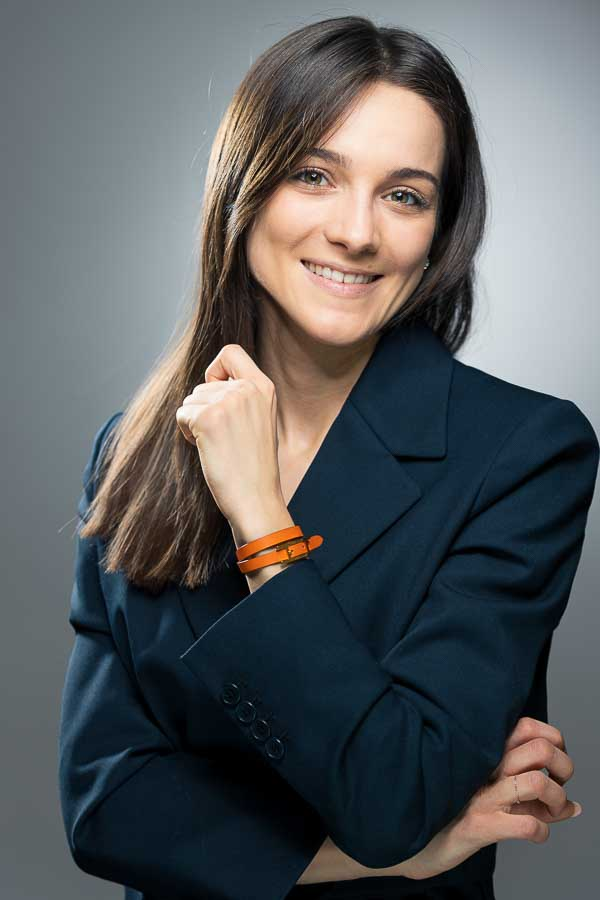
\includegraphics[width=0.3\textwidth]{clara.jpg}
\end{figure}

\begin{itemize}
    \item \textbf{Âge} : 29 ans
    \item \textbf{Profession} : Infirmière
    \item \textbf{Localisation} : Montpellier
    \item \textbf{Objectif} : Trouver un véhicule fiable, économe et adapté à un usage urbain
    \item \textbf{Comportement} :
    \begin{itemize}
        \item Recherche un véhicule d’occasion dans un budget de 12 000 à 15 000 euros
        \item Privilégie la consommation, la taille et le confort plutôt que la puissance
        \item Hésite entre plusieurs modèles et souhaite comparer les options selon ses critères
    \end{itemize}
    \item \textbf{Besoins couverts par AutoPredict} :
    \begin{itemize}
        \item Accéder à une sélection de modèles filtrés selon ses préférences
        \item Comprendre la variation des prix en fonction des caractéristiques sélectionnées
    \end{itemize}
\end{itemize}

\chapter{Caractéristiques Principales}
\section{Interface Conviviale}
L’interface utilisateur est conçue avec ReactJS pour offrir une navigation fluide et interactive.
L’accent est mis sur l’ergonomie, la clarté des résultats et la facilité d’utilisation même pour des utilisateurs non-experts.


\section{Sources Fiables}
Les données utilisées proviennent de datasets publics sur les voitures, incluant des caractéristiques techniques (puissance, consommation, taille, style), économiques (prix, popularité), et temporelles (année de sortie).

\chapter{Architecture métier}
\section{Frontend}
Le frontend est développé en ReactJS. Il intègre des composants interactifs permettant à l’utilisateur de :

\begin{itemize}
    \item Rechercher des modèles de voitures correspondant à ses critères et à son budget
    \item Estimer la valeur d’un véhicule en fonction de caractéristiques spécifiques
    \item Visualiser graphiquement les résultats obtenus (filtres, comparateurs, graphiques de prix, etc.)
\end{itemize}

L’interface dialogue avec le backend via une API REST.


\section{Backend}
Le backend est conçu en Python à l’aide du framework Flask. Il gère :

\begin{itemize}
    \item L’accès à la base NoSQL contenant les données automobiles
    \item L’exécution des modèles de machine learning pour la recommandation de véhicules et l’estimation des prix
    \item L’interface avec le frontend via une API structurée
\end{itemize}

Les requêtes utilisateurs sont traitées dynamiquement pour retourner des résultats adaptés et rapides.


\section{Base de données}
La base de données utilisée est de type NoSQL, permettant une flexibilité dans la gestion des formats de données hétérogènes typiques du domaine automobile.

\chapter{Architecture distribuée}
\section{Application Hosting}
Le projet est conteneurisé afin de faciliter le déploiement, la scalabilité et la portabilité. Docker est utilisé pour packager les composants.

\section{Database Hosting}
La base NoSQL est hébergée dans un environnement compatible cloud. Elle stocke les jeux de données enrichis et traités, accessibles via API.

\chapter{Pratiques de Collaboration et de DevOps}
\section{Project Management}
Le projet est géré en équipe de trois membres : Frédéric, Yann et Jérémy. Le suivi des tâches se fait de manière collaborative autour d'outils de gestion agile.

\section{Versionnement}
L’ensemble du code source est versionné via Git, avec des dépôts organisés pour le frontend, le backend et les notebooks d'analyse/ML.

\section{Intégration Continue et Déploiement Continu}
Des pipelines CI/CD seront mis en place pour automatiser les tests, le linting, et le déploiement sur l’environnement de développement.

\section{Maintenabilité du code}
L'utilisation de conteneurs, de frameworks standards (Flask, React) et de pratiques de développement modulaire assure la maintenabilité du projet.

\section{Qualité du code}
Le code est documenté, typé et validé avec des outils de linting et des tests unitaires, notamment sur les scripts de preprocessing et les modèles ML.

\chapter{Partie Data Analytique}

\thispagestyle{plain}
\pagestyle{plain}


\section{Analyse de données}

\subsection{Préparation et nettoyage des données}

La phase de préparation a consisté à rendre les données cohérentes, complètes et prêtes à être visualisées. Elle s’est déroulée comme suit :

\begin{itemize}
  \item \textbf{Standardisation} : Uniformisation des noms de colonnes en minuscules avec des underscores pour assurer une manipulation fluide.
  \item \textbf{Suppression des doublons} : Élimination des entrées redondantes basées sur les identifiants véhicule/modèle.
  \item \textbf{Traitement des valeurs manquantes} :
    \begin{itemize}
        \item Remplacement par des valeurs par défaut ou par la moyenne (ex. nombre de portes ou de cylindres).
        \item Suppression des lignes avec des données critiques absentes.
    \end{itemize}
  \item \textbf{Filtrage des transmissions inconnues} : Les entrées comportant `UNKNOWN` pour la transmission ont été exclues de l’analyse.
  \item \textbf{Création de nouvelles variables} :
    \begin{itemize}
        \item Quantiles de prix (MSRP) pour catégoriser les véhicules.
        \item Plages de puissance moteur pour les regrouper en catégories (`faible`, `moyenne`, `élevée`, etc.).
        \item Calcul de la consommation moyenne combinée (ville + autoroute).
    \end{itemize}
\end{itemize}

\subsection{Présentation des graphiques et interprétation}

Dans cette section, nous explorons différentes visualisations de données afin d’extraire des tendances structurelles sur notre flotte de véhicules. Chaque graphique est accompagné d’une interprétation opérationnelle, utile pour guider les recommandations clients.

\paragraph{1. Répartition des types de transmission selon les quantiles de prix}\mbox{}

\begin{figure}[H]
\centering
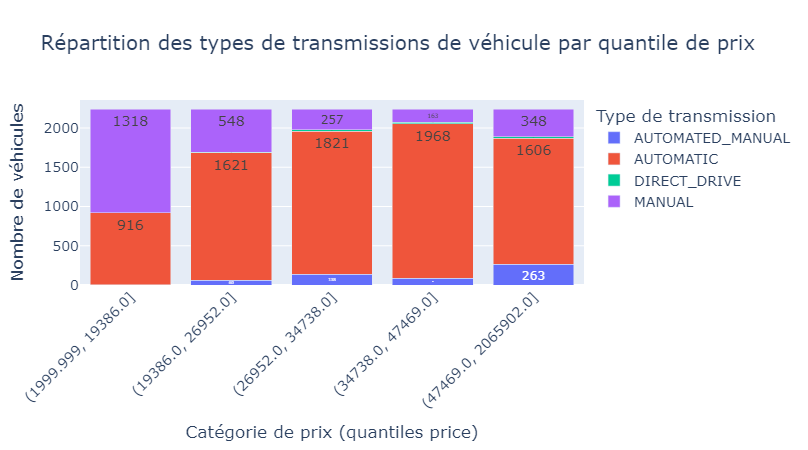
\includegraphics[width=0.8\textwidth]{transmission_vs_price.png}
\caption{Répartition des transmissions par tranche de prix (quantiles MSRP)}
\end{figure}


Ce graphique à barres empilées montre que :
\begin{itemize}
  \item Les transmissions \textbf{automatiques} dominent très largement dans les gammes de prix \textit{intermédiaires à élevées}, représentant parfois plus de \textbf{80 \%} des véhicules.
  \item Les transmissions \textbf{manuelles} sont surtout présentes dans les véhicules du \textit{premier quantile de prix}, et disparaissent progressivement à mesure que le prix augmente.
  \item Les transmissions \textbf{automatisées manuelles} sont rares, présentes essentiellement dans des véhicules haut de gamme ou spécifiques.
\end{itemize}

Cette distribution illustre un lien direct entre la gamme tarifaire et le type de confort/conduite attendu.

\paragraph{2. Répartition des styles de véhicules selon le type de transmission}\mbox{}

\begin{figure}[H]
\centering
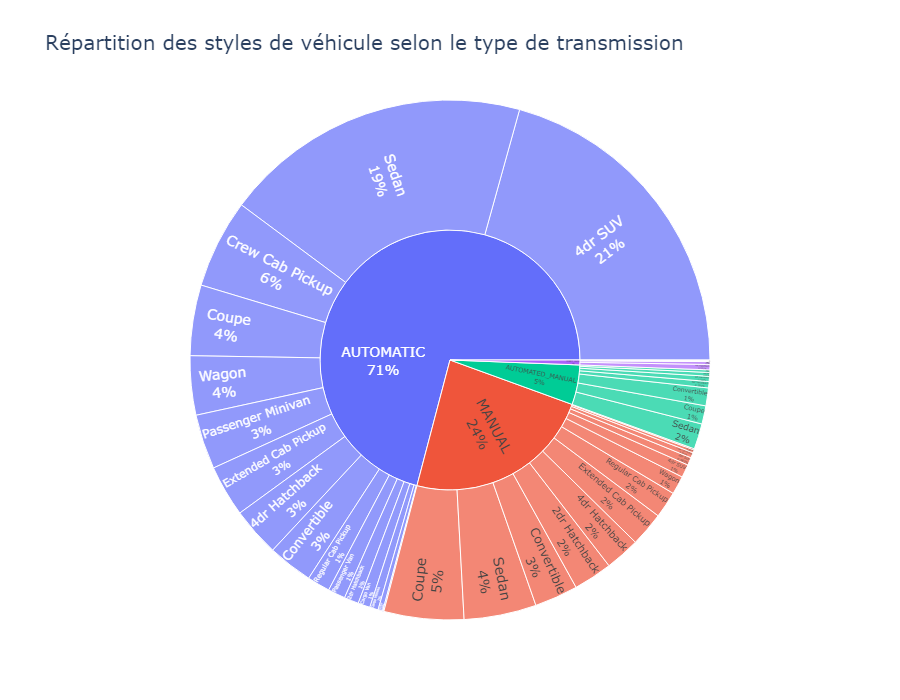
\includegraphics[width=0.8\textwidth]{transmission_style_sunburst.png}
\caption{Répartition des styles de véhicule selon la transmission}
\end{figure}

Le diagramme sunburst confirme les tendances précédentes :
\begin{itemize}
  \item Les \textbf{SUV} et \textbf{berlines (sedan)} sont principalement associés aux transmissions automatiques, répondant à des besoins de confort et d’usage urbain/familial.
  \item Les \textbf{coupés}, \textbf{hatchbacks} ou \textbf{pickups} sont souvent en transmission manuelle, adaptés à des usages économiques, sportifs ou professionnels.
  \item Les transmissions rares comme \texttt{DIRECT\_DRIVE} restent anecdotiques.
\end{itemize}

\paragraph{3. Consommation moyenne selon puissance moteur et cylindres}\mbox{}

\begin{figure}[H]
\centering
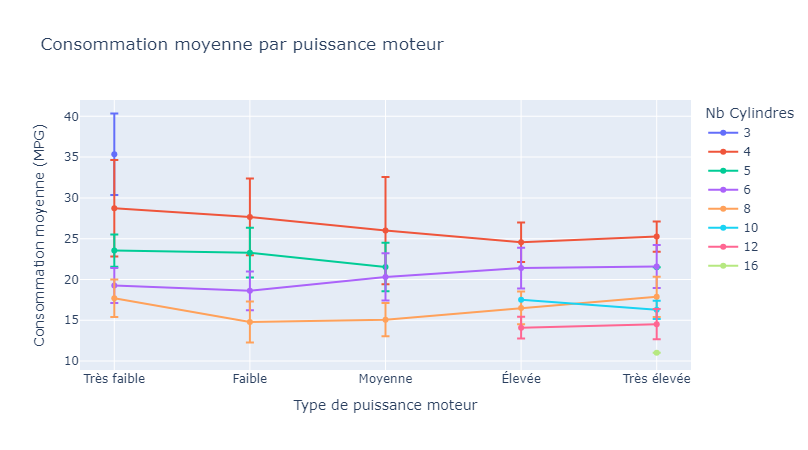
\includegraphics[width=0.8\textwidth]{hp_vs_cylinders.png}
\caption{Consommation moyenne selon puissance moteur et nombre de cylindres}
\end{figure}

On observe une relation logique entre la puissance du moteur et la consommation :
\begin{itemize}
  \item Les véhicules à \textbf{puissance très élevée} et \textbf{8 cylindres ou plus} affichent une consommation moyenne plus élevée.
  \item Les modèles à \textbf{puissance moyenne à faible} ont des consommations plus stables et optimisées.
  \item Cette analyse permet de recommander les modèles selon un compromis performance/efficacité.
\end{itemize}

\paragraph{4. Prix moyen par catégorie de véhicule et puissance moteur}\mbox{}

\begin{figure}[H]
\centering
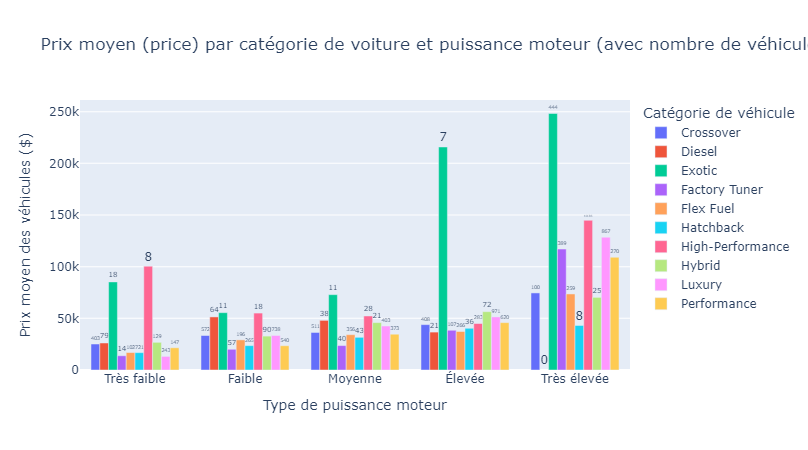
\includegraphics[width=0.9\textwidth]{price_vs_hp_market.png}
\caption{Prix moyen par catégorie de voiture et puissance moteur (avec nombre de véhicules)}
\end{figure}

Cette visualisation en barres groupées révèle :
\begin{itemize}
  \item Les véhicules \textbf{exotiques} dominent dans les plages de puissance élevée avec un prix moyen largement supérieur à 200 000\$.
  \item La catégorie \textbf{haut de gamme (Luxury)} est répartie sur toutes les puissances, mais fortement concentrée sur les plages hautes.
  \item Les \textbf{véhicules hybrides, diesel, flex fuel} et \textbf{compactes (Hatchback)} occupent les plages basses à moyennes, avec des prix accessibles.
\end{itemize}

Ce graphique complète la compréhension des segments en croisant l’offre produit avec les puissances moteur disponibles.

\paragraph{5. Profil d’achat et recommandations commerciales}\mbox{}

\vspace{0.5cm}

À partir de l’ensemble de ces analyses, plusieurs profils-types émergent :
\begin{itemize}
  \item Un \textbf{client urbain familial}, à la recherche de confort et de fiabilité, sera orienté vers un \textbf{SUV automatique} de gamme intermédiaire.
  \item Un \textbf{client professionnel ou rural} peut viser un \textbf{pickup manuel}, robuste et économique.
  \item Un \textbf{jeune conducteur ou petit budget} sera conseillé vers un \textbf{coupé ou hatchback manuel}, situé dans les premiers quantiles de prix.
  \item Pour les \textbf{amateurs de performance ou de véhicules hybrides}, on oriente vers des modèles à forte puissance ou technologies spécifiques, tout en tenant compte du marché (exotic, performance, luxury).
\end{itemize}

L’approche analytique appliquée à nos données permet donc d’alimenter directement notre moteur de recommandation personnalisé.


\subsection{Analyse de la diversification de marque et de modèle}

\subsubsection{Volume de modèles distincts par constructeur}

\begin{figure}[H]
    \centering
    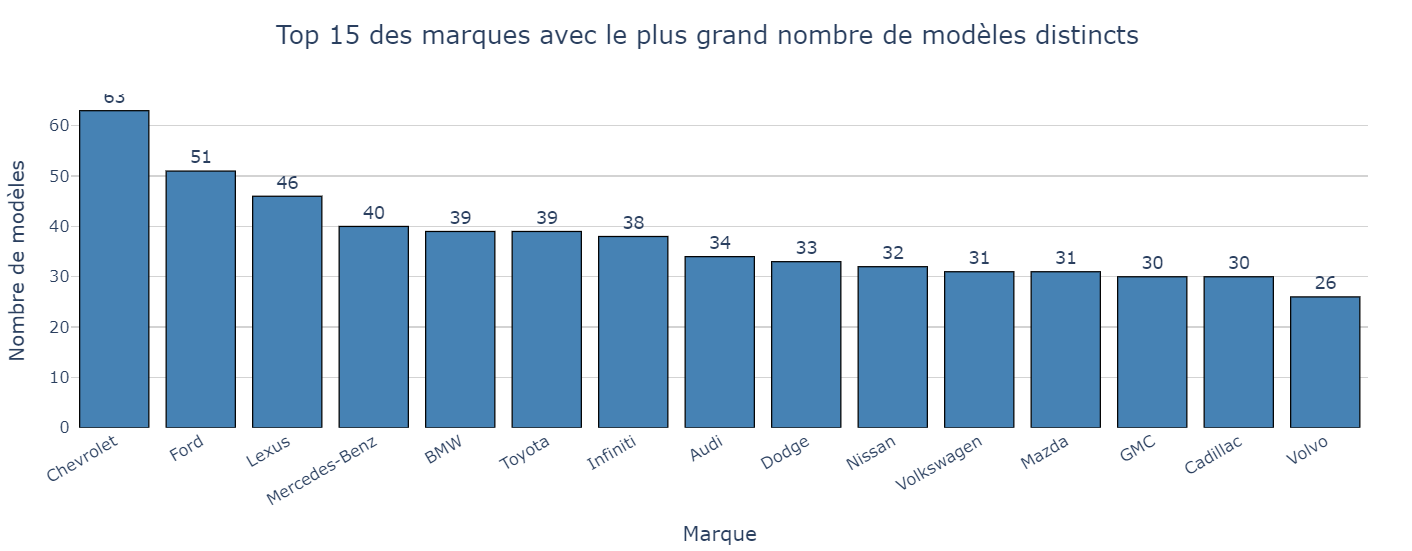
\includegraphics[width=1\textwidth]{Modele_marque.png}
    \caption{Top 15 des marques avec le plus grand nombre de modèles distincts}
    \label{fig:modele-marque}
\end{figure}

Ce premier graphique dresse un panorama des marques les plus présentes sur le marché en termes de diversité de modèles proposés. On y observe que \textbf{Chevrolet} domine le classement avec 63 modèles, suivi de \textbf{Ford} avec 51 modèles. Ces deux constructeurs américains adoptent une stratégie résolument généraliste, en multipliant les déclinaisons afin de toucher une clientèle très large.

Derrière eux, on retrouve \textbf{Lexus}, \textbf{Mercedes-Benz} et \textbf{BMW}, dont les catalogues sont également étoffés mais plus orientés vers le haut de gamme. Cette diversité traduit une volonté de capter des niches plus spécifiques, en multipliant les combinaisons de finitions, de motorisations et de segments.

Ainsi, ce classement met en lumière deux stratégies différentes : 
\begin{itemize}
    \item une logique de volume (Chevrolet, Ford) pour occuper tous les segments du marché,
    \item une logique de spécialisation (Lexus, BMW, Mercedes-Benz) avec une forte présence dans le premium.
\end{itemize}

\subsubsection{Répartition des segments pour les principales marques}

\begin{figure}[H]
    \centering
    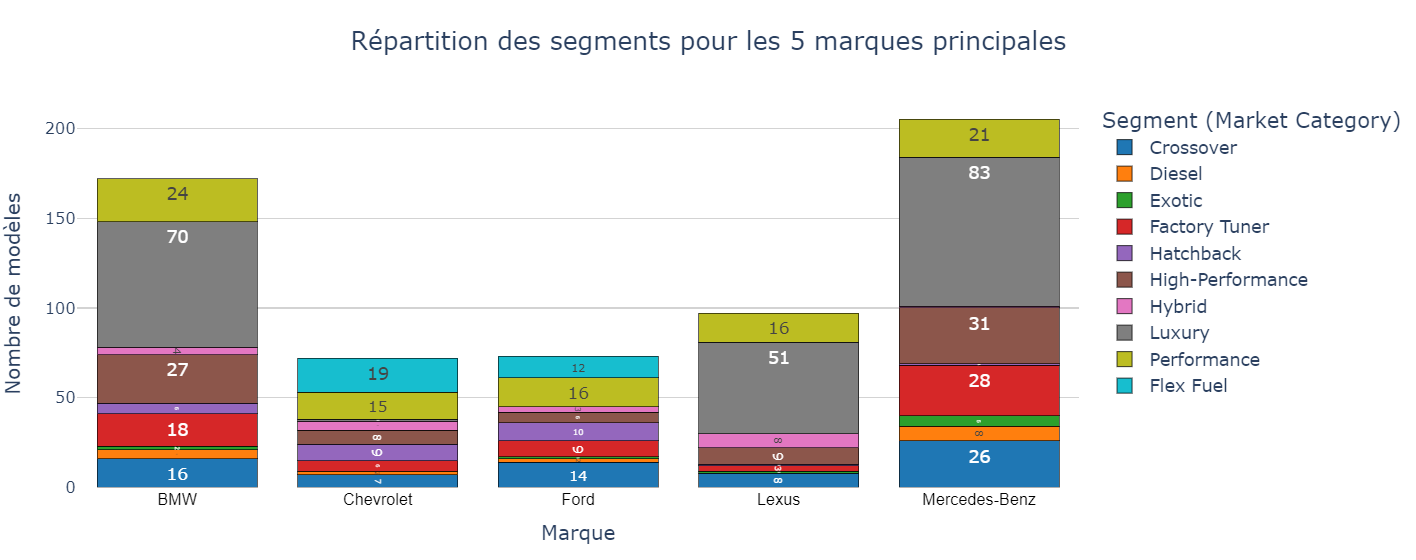
\includegraphics[width=1\textwidth]{Marque_nbmodele.png}
    \caption{Répartition des segments pour les 5 marques principales}
    \label{fig:marque-nbmodele}
\end{figure}

Ce second graphique affine la lecture précédente en détaillant la composition des catalogues des cinq marques les plus prolifiques. Plusieurs enseignements clés en ressortent :

\begin{itemize}
    \item \textbf{Mercedes-Benz} affiche une présence remarquable dans la majorité des segments, en particulier dans le \textit{Luxury} (83 modèles), mais aussi dans le \textit{Performance}, le \textit{Crossover} ou encore le \textit{Factory Tuner}. Ce spectre très large traduit une stratégie ambitieuse, capable de séduire aussi bien les amateurs de confort que de performance.
    
    \item \textbf{BMW} suit une trajectoire similaire, avec une prédominance du segment \textit{Luxury} (70 modèles), mais aussi une forte présence dans les segments dynamiques comme le \textit{High-Performance}.

    \item \textbf{Chevrolet} et \textbf{Ford}, bien que moins focalisés sur le haut de gamme, offrent une répartition beaucoup plus homogène entre les différents segments, ce qui illustre leur orientation généraliste. Ils se démarquent notamment par leur présence significative dans les catégories \textit{Crossover}, \textit{Flex Fuel} ou \textit{Hatchback}.

    \item Enfin, \textbf{Lexus} adopte une position intermédiaire : fortement ancrée sur le segment \textit{Luxury} (51 modèles), la marque japonaise complète son offre avec des incursions dans le \textit{Hybrid}, le \textit{Performance} et le \textit{Crossover}, tout en conservant un positionnement qualitatif.
\end{itemize}

\subsubsection{Diversité de segments et popularité moyenne des marques}

\begin{figure}[H]
    \centering
    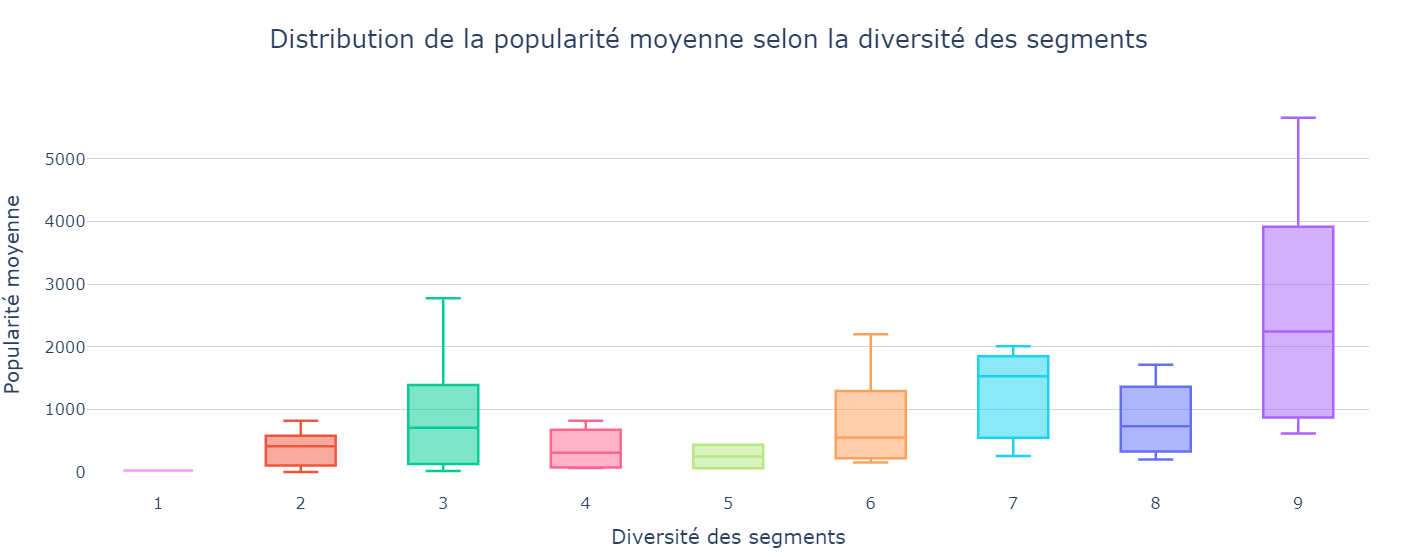
\includegraphics[width=1\textwidth]{Section_pop.png}
    \caption{Distribution de la popularité moyenne selon la diversité des segments}
    \label{fig:section-pop}
\end{figure}

Ce dernier graphique aborde la question sous un autre angle : la diversité de l’offre est-elle un levier efficace pour accroître la notoriété ou l’attractivité d’une marque ?

On remarque que les marques présentes dans peu de segments (entre 1 et 3) affichent généralement une popularité moyenne faible, avec peu de dispersion. Cela traduit une spécialisation qui, bien que cohérente, reste limitée en termes d’audience.

À partir de 6 segments couverts, on constate une augmentation significative de la popularité moyenne, mais aussi une forte dispersion. Certaines marques diversifiées explosent en popularité, tandis que d’autres, malgré une offre étendue, peinent à s’imposer. Le message est donc nuancé : la diversification est souvent une condition favorable à la visibilité, mais ne garantit pas à elle seule le succès commercial.

\subsubsection{Enseignements pour le moteur AutoPredict}

Ces différentes visualisations apportent des éléments précieux pour l’algorithme de recommandation :

\begin{itemize}
    \item Une marque très diversifiée comme Mercedes-Benz peut convenir à des profils très variés. Elle est donc intéressante à proposer dans des contextes où les préférences de l’utilisateur ne sont pas encore clairement établies.
    \item À l’inverse, une marque spécialisée dans le haut de gamme ou les performances (comme BMW ou Lexus) pourra être suggérée à des utilisateurs plus ciblés, ayant exprimé des attentes spécifiques.
    \item Enfin, la diversité de segments est un bon indicateur de flexibilité commerciale : intégrer cette variable dans AutoPredict permettra d’anticiper le champ des possibles qu’une marque peut offrir à un utilisateur donné.
\end{itemize}

Ainsi, cette analyse souligne l’importance d’adapter les suggestions non seulement en fonction des caractéristiques techniques des modèles, mais aussi selon la stratégie commerciale des constructeurs.


\subsection{Analyse de la dépréciation}

\subsubsection{ Dépréciation moyenne des véhicules par année}
\begin{figure}[H] \centering 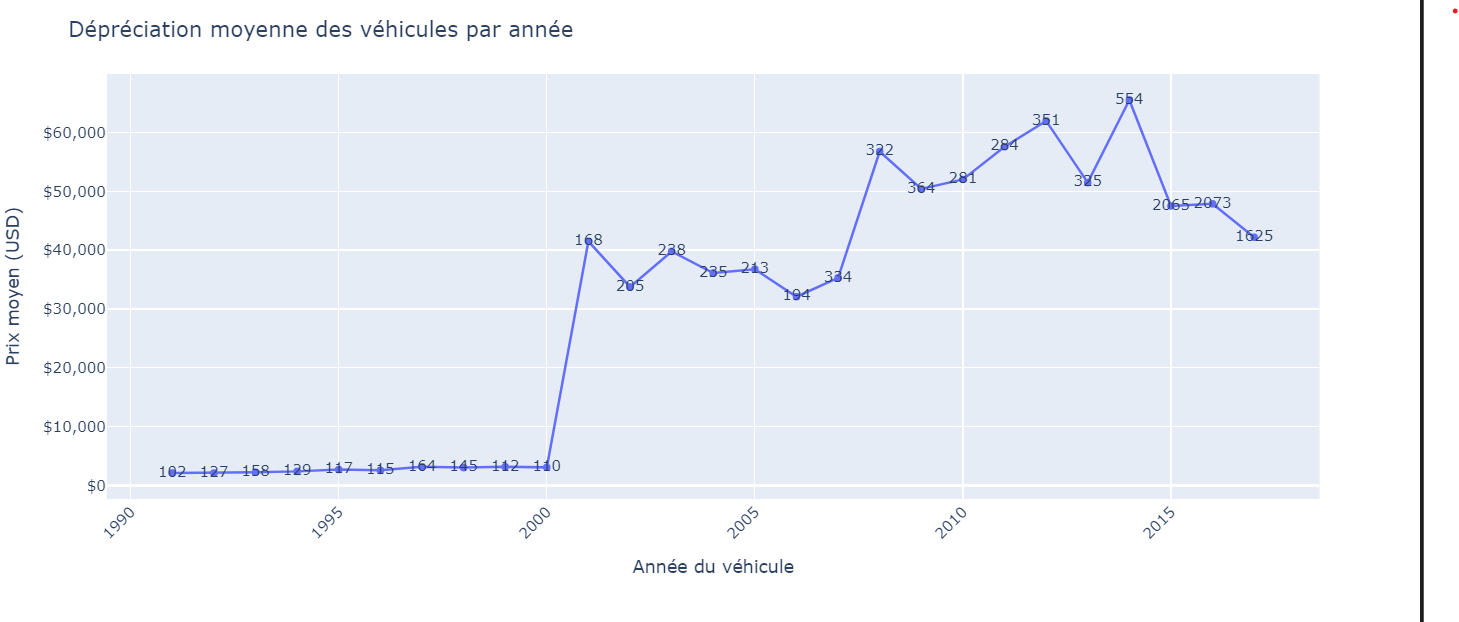
\includegraphics[width=1\textwidth]{Annee_prix.png} \caption{Dépréciation moyenne des véhicules par année} \label{fig:annee-prix} \end{figure}

Ce graphique représente l’évolution du prix moyen des véhicules en fonction de leur année de fabrication. Il permet d’observer le phénomène de dépréciation sur le long terme, en regroupant aussi bien des véhicules neufs que d’occasion.

\textbf{Analyse détaillée :} \begin{itemize} \item Les modèles antérieurs à l’an 2000 présentent une valeur résiduelle très faible, majoritairement inférieure à 10 000 dollars. Cette tendance s’explique par une accumulation de kilomètres, une usure plus marquée et une inadéquation technologique avec les normes actuelles. \item Une baisse brutale du prix moyen est visible entre les années 2000 et 2002. Cette rupture peut coïncider avec des politiques environnementales ou fiscales incitatives au renouvellement du parc automobile. \item À partir de 2005, on observe une courbe ascendante continue du prix moyen des véhicules, atteignant un pic autour de 2014. Cela reflète probablement une montée en gamme du marché (meilleur équipement, technologies embarquées, électrification partielle...). \end{itemize}

\textbf{Conclusion :}
La valeur d’un véhicule chute rapidement durant les 10 à 15 premières années après sa sortie d’usine. Passé ce cap, la décote se stabilise à des niveaux très bas. Ces observations confirment qu’il peut être peu rentable, économiquement, d’acheter un véhicule trop ancien — en particulier en l'absence de fiabilité ou de revalorisation possible.

\subsubsection{Dépréciation par style de véhicule}
\begin{figure}[H] \centering \includegraphics[width=1\textwidth]{année_pris_dep.png} \caption{Dépréciation par style de véhicule} \label{fig:annee-pris-dep} \end{figure}

Ce graphique explore la manière dont le style de carrosserie influence le prix moyen d’un véhicule au fil du temps. Chaque courbe correspond à un type de style (SUV, coupé, van, etc.).

\textbf{Constats notables :} \begin{itemize} \item Les \textit{SUV 4 portes}, \textit{Convertibles} et \textit{Crew Cab Pickups} conservent une valeur relativement stable, souvent au-dessus de 50 000 dollars. Cette rétention de valeur témoigne de leur attractivité constante sur le marché, même en occasion. \item À l’inverse, les \textit{Cargo Vans}, \textit{2dr Hatchbacks} ou encore les \textit{Sedans} restent globalement en dessous de 20 000 dollars, traduisant une moindre demande ou un usage plus utilitaire. \item Le cas particulier des \textit{Convertible SUV} est à souligner : malgré leur rareté, ces modèles enregistrent des pics de prix dépassant 100 000 dollars. Leur rareté et leur image de niche haut de gamme expliquent cette valorisation atypique. \end{itemize}

\textbf{Interprétation :}
Les styles qui véhiculent un imaginaire de plaisir (convertible, SUV, pickup) ou de statut conservent mieux leur prix que ceux purement fonctionnels. La perception sociale et l'usage projeté semblent donc peser lourdement dans la dépréciation d’un véhicule.

\subsubsection{Dépréciation par catégorie marketing}
\begin{figure}[H] \centering 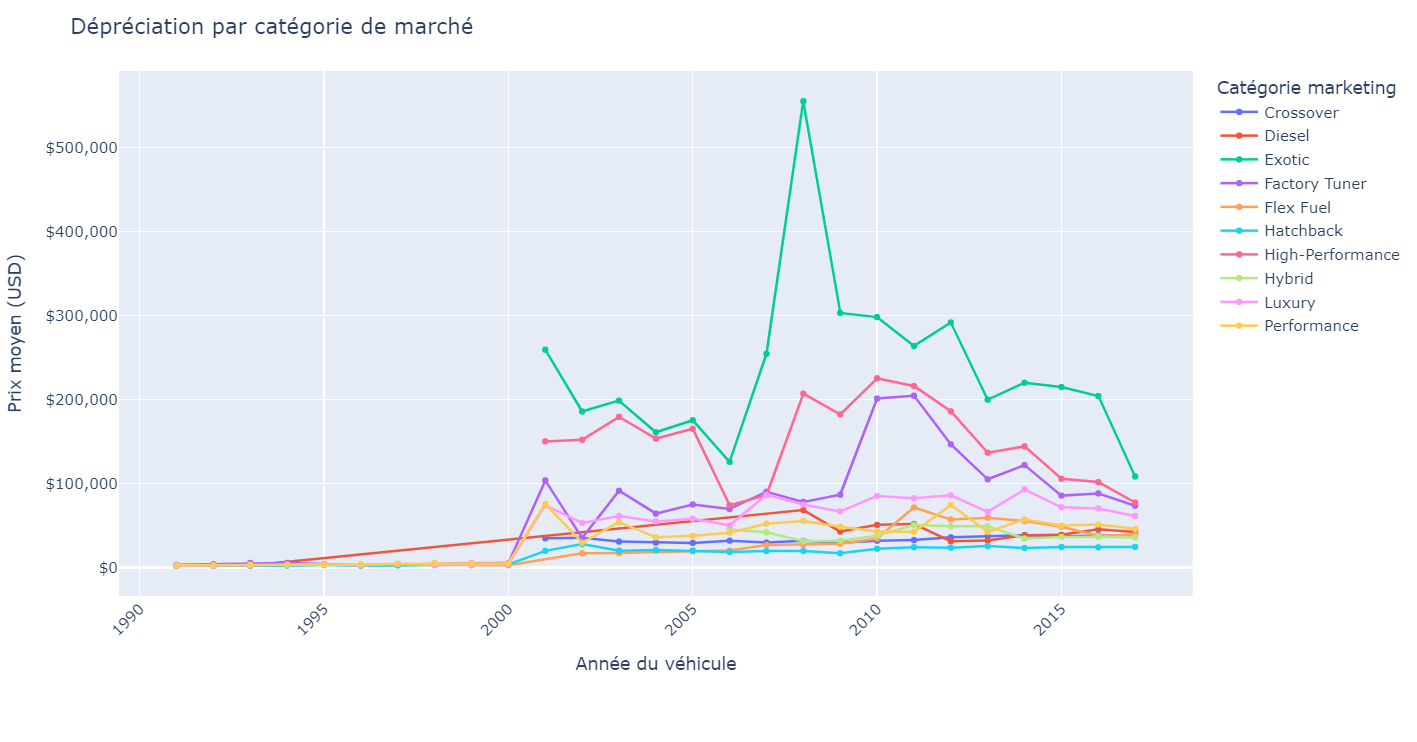
\includegraphics[width=1\textwidth]{annee_prix_cat.png} \caption{Dépréciation par catégorie marketing} \label{fig:annee-prix-cat} \end{figure}

Ici, le graphique fait le lien entre la catégorie marketing d’un véhicule (Luxury, Hybrid, Diesel, etc.) et l’évolution de sa valeur au fil du temps.

\textbf{Tendances principales :} \begin{itemize} \item Les véhicules classés \textit{Exotic}, \textit{High-Performance} ou \textit{Luxury} dominent en termes de prix moyen. Ces segments dépassent largement les 60 000 dollars, et certains modèles de niche (ex : Exotic) peuvent frôler ou dépasser les 500 000 dollars. \item Les véhicules à vocation économique ou utilitaire comme les \textit{Flex Fuel}, \textit{Diesel} ou \textit{Hatchback} restent dans une fourchette basse (en dessous de 30 000 dollars), avec une décroissance régulière. \item Le segment \textit{Crossover} se démarque : il affiche une très bonne stabilité, avec des prix moyens compétitifs et peu de chute marquée. Sa polyvalence et sa modernité en font un style très recherché. \end{itemize}

\textbf{Ce que cela révèle :}
La dépréciation est fortement corrélée à la manière dont un véhicule est positionné. Plus l’image est prestigieuse, rare ou technologique, plus la valeur est préservée. À l’inverse, un véhicule perçu comme « utilitaire » est souvent plus sujet à l’obsolescence perçue.
\vspace{0.5em}
\textbf{Interprétation globale :}
\begin{itemize}
    \item La catégorie marketing influence fortement la rétention de valeur : les modèles haut de gamme, performants ou hybrides sont mieux valorisés dans le temps.
    \item À l’inverse, les véhicules à vocation pratique ou économique, bien qu’utiles, perdent plus rapidement de leur valeur.
\end{itemize}

\vspace{1em}
Ces résultats confirment que la perception du véhicule joue un rôle central dans sa valeur résiduelle. Intégrer cette information dans le moteur de recommandation d'AutoPredict permet d’adapter les suggestions aux attentes des utilisateurs, en tenant compte de leur sensibilité au prestige, à la performance ou à l’économie.

\chapter{Partie Machine Learning}

\thispagestyle{plain}
\pagestyle{plain}

\section{Objectif et Intégration}

La composante \textit{Machine Learning} du projet \textbf{AutoPredict} a pour objectif de fournir une fonctionnalité intelligente essentielle : 
\begin{itemize}
    \item \textbf{L'estimation du prix} de véhicules d'occasion en fonction de leurs caractéristiques techniques.
\end{itemize}

Cette estimation s'adresse principalement à un utilisateur se plaçant dans la peau d’un vendeur souhaitant connaître la valeur de revente potentielle de son véhicule. L’intégration de cette composante permet ainsi de proposer un service à forte valeur ajoutée, en facilitant la prise de décision pour les particuliers ou les professionnels.
Le code est disponible dans le notebooks \texttt{AutoPredict\_ML.ipynb}. 
\newline
\newline
\subsection{Démarche générale du projet}
Notre projet suit une démarche structurée en trois grandes phases, inspirée des bonnes pratiques en Machine Learning. Cette méthodologie nous a permis de passer de données brutes à la construction d'un moteur de recommandation intelligent.

\begin{itemize}
    \item \textbf{Pré-traitement des données} :
    \begin{itemize}
        \item \textit{Formalisation des objectifs} : définition claire des besoins utilisateurs.
        \item \textit{Acquisition des données} : collecte et consolidation de données (prix, caractéristiques techniques, type de transmission, consommation, etc.).
        \item \textit{Préparation des données} : nettoyage, standardisation, encodage des variables catégorielles, et normalisation des variables numériques.
    \end{itemize}
    
    \item \textbf{Phase d'apprentissage} :
    \begin{itemize}
        \item \textit{Apprentissage supervisé} : application d'algorithmes de Machine Learning pour estimer les prix et recommander des modèles de véhicules adaptés.
        \item \textit{Sélection des méthodes} : utilisation de techniques adaptées comme la Classification, les k-plus proches voisins (KNN) ou encore les réseaux de neuronnes (RNN).
    \end{itemize}
    
    \item \textbf{Post-traitement et validation} :
    \begin{itemize}
        \item \textit{Évaluation et validation} : mesure de la qualité des prédictions à l'aide d'indicateurs.
        \item \textit{Interprétation des résultats} : analyse fine pour tirer des conclusions concrètes sur les préférences et tendances de marché.
    \end{itemize}
\end{itemize}

Cette démarche rigoureuse garantit la fiabilité, la pertinence et l'interprétabilité de notre solution AutoPredict, tout en restant alignée avec les attentes pratiques du domaine automobile.

\subsection{Choix de l'approche d'apprentissage}

Dans le cadre de notre projet, l'objectif est de réaliser des prédictions sur les caractéristiques et les prix des véhicules. Cette problématique nous oriente naturellement vers l'apprentissage supervisé, car nous disposons d'un ensemble de données étiquetées, c'est-à-dire que pour chaque véhicule, les informations réelles (prix, caractéristiques, etc.) sont connues.

L'apprentissage supervisé est une branche du Machine Learning où un modèle est entraîné à partir d'exemples étiquetés afin de prédire une sortie pour de nouvelles données. Lorsque la variable cible est discrète (appartenance à une classe ou à une catégorie), on parle alors de classification.

Dans notre cas, comme nous cherchons à recommander ou positionner des véhicules selon différentes catégories de critères (par exemple style, segment de marché), la tâche est assimilable à un problème de classification supervisée.

Ainsi, notre démarche s'appuie sur :
\begin{itemize}
    \item l'utilisation de données historiques étiquetées,
    \item la mise en œuvre d'algorithmes de classification pour associer de nouveaux véhicules à la bonne catégorie ou prédire des préférences d'achat.
\end{itemize}

\subsection{Présentation des modèles utilisés}

Dans le cadre de notre projet de prédiction automobile, nous avons choisi d'expérimenter trois types de modèles complémentaires, chacun ayant des avantages spécifiques en fonction de la nature des données et des objectifs visés. Voici une brève présentation de chacun :

\subsubsection{Random Forest}

La \textbf{Random Forest} est un algorithme d'ensemble basé sur la combinaison de plusieurs arbres de décision. Chaque arbre est entraîné sur un sous-échantillon différent des données, et les prédictions finales sont obtenues par un vote majoritaire (pour la classification) ou une moyenne (pour la régression). Ce modèle est reconnu pour sa robustesse, sa capacité à réduire le surapprentissage (overfitting) par rapport à un arbre unique, et son efficacité sur des ensembles de données complexes et bruités.

\subsubsection{K-Nearest Neighbors (KNN)}

Le \textbf{K-Nearest Neighbors} est un algorithme simple mais puissant qui classe un nouvel échantillon en fonction des $k$ exemples les plus proches dans l'espace des caractéristiques. Lorsque le nombre de voisins $k$ est faible, le modèle peut être extrêmement précis, car il s'adapte très finement aux données locales. Cependant, un $k$ trop petit risque de rendre le modèle très sensible au bruit et de provoquer un phénomène de surapprentissage (\textit{overfitting}). À l'inverse, un $k$ plus élevé rend le modèle plus généraliste, mais au prix d'une perte de précision locale.

\subsubsection{Réseaux de Neurones (RNN)}

Les \textbf{Réseaux de Neurones} constituent une approche inspirée du fonctionnement biologique du cerveau humain. Dans notre projet, nous explorons une architecture simple de réseau de neurones (de type dense) pour la prédiction. Les réseaux de neurones sont capables de modéliser des relations complexes entre les variables, en combinant plusieurs couches de traitement non linéaires. Bien que plus coûteux en temps de calcul et nécessitant davantage de données pour éviter l'overfitting, ils offrent une grande flexibilité et une capacité d'adaptation sur des problèmes de prédiction riches en interactions entre variables.



\subsection{Indicateurs de performance utilisés}

Afin d’évaluer la qualité des prédictions réalisées par nos modèles, nous avons utilisé deux métriques principales vuent en cours : le coefficient de détermination \( R^2 \) et la racine de l’erreur quadratique moyenne (RMSE).

\subsubsection*{Coefficient de détermination (\( R^2 \))}

Le \( R^2 \) mesure la proportion de la variance de la variable cible qui est expliquée par le modèle. 
\begin{itemize}
    \item \( R^2 = 1 \) : le modèle explique parfaitement les données.
    \item \( R^2 = 0 \) : le modèle n'explique pas mieux que la moyenne.
    \item \( R^2 < 0 \) : le modèle est pire qu'une simple moyenne.
\end{itemize}

Un \( R^2 \) élevé indique donc que le modèle ajuste correctement les données.

\subsubsection*{Racine de l'erreur quadratique moyenne (RMSE)}

La RMSE évalue l'écart moyen entre les valeurs prédites et les valeurs observées. 
\begin{itemize}
    \item Une RMSE faible indique que les prédictions du modèle sont proches des valeurs observées.
    \item Contrairement à \( R^2 \), la RMSE est exprimée dans la même unité que la variable prédite (ici le prix en dollars).
\end{itemize}

La combinaison de \( R^2 \) et de la RMSE nous permet d’obtenir une vision complète de la performance : précision globale et écart moyen en valeur absolue.

\subsection{Surapprentissage et sous-apprentissage}

Dans notre projet AutoPredict, afin de mesurer la qualité de nos modèles, nous nous appuyons principalement sur deux indicateurs : le RMSE (Root Mean Squared Error) et le R\textsuperscript{2} (coefficient de détermination). Ces deux métriques nous permettent également de détecter deux phénomènes courants en machine learning : le surapprentissage (overfitting) et le sous-apprentissage (underfitting).

\subsubsection{Overfitting (Surapprentissage)}

Le \textbf{surapprentissage} survient lorsque le modèle est trop spécialisé sur les données d'entraînement. Il présente alors un \textbf{RMSE très faible} et un \textbf{R\textsuperscript{2} élevé} sur l'ensemble d'entraînement, mais ses performances chutent fortement sur l'ensemble de test. 

Dans notre contexte, nous considérons qu'il y a overfitting si :
\begin{itemize}
    \item La différence de RMSE entre l'entraînement et le test dépasse \textbf{15\%}.
    \item Le R\textsuperscript{2} sur le test est inférieur de plus de \textbf{0.1} par rapport à celui obtenu sur l'entraînement.
\end{itemize}

Cela signifie que le modèle a "mémorisé" les données au lieu d'apprendre à généraliser.

\subsubsection{Underfitting (Sous-apprentissage)}

Le \textbf{sous-apprentissage} se produit lorsque le modèle est incapable de capturer la structure des données, que ce soit sur l'entraînement ou sur le test. Cela se traduit par un \textbf{RMSE élevé} sur les deux jeux de données et un \textbf{R\textsuperscript{2} faible}.

Nous détectons un underfitting si :
\begin{itemize}
    \item Le RMSE est élevé et proche entre l'entraînement et le test.
    \item Le R\textsuperscript{2} reste inférieur à \textbf{0.6} sur les deux ensembles.
\end{itemize}

Cela indique que notre modèle est trop simple pour le problème posé.

\subsubsection{Objectif d'équilibre}

Un bon modèle doit trouver un \textbf{équilibre} :
\begin{itemize}
    \item Un \textbf{RMSE bas} et similaire entre l'entraînement et le test.
    \item Un \textbf{R\textsuperscript{2} élevé} (idéalement supérieur à 0.7), avec peu d'écart entre les deux ensembles.
\end{itemize}

C'est en surveillant en parallèle RMSE et R\textsuperscript{2} que nous pouvons ajuster correctement nos hyperparamètres pour éviter ces deux dérives et garantir un modèle à la fois précis et généralisable.



\section{Préparation des Données}

\subsection{Nettoyage}

Avant l'entraînement du modèle, un travail de préparation minutieux a été réalisé, avec des étapes spécifiques par rapport à l'analyse des données :
\begin{itemize}
    \item \textbf{Nettoyage des doublons et des valeurs manquantes}. Nous avons décidé de supprimer les colonnes présentant un nombre élevé de valeurs manquantes pour éviter la suppression d'un trop grand nombre de lignes. Par exemple, la colonne "market" comportait 3376 valeurs manquantes sur un total de 11914 lignes et a donc été supprimée. La colonne "popularité" a également été retirée car elle n'était pas pertinente pour la suite.
    \item \textbf{Standardisation des noms de colonnes} pour faciliter leur manipulation, certains noms n'étant pas suffisamment explicites.
    \item \textbf{Regroupement de plusieurs catégories en une}. Dans la colonne du type de carburant, nous avons regroupé les nombreuses catégories en six grandes catégories (essence, flex fuel, électrique, diesel, gaz naturel et autre). Cela sera particulièrement utile pour l'interface utilisateur (UI).
    \item \textbf{Suppression des outliers}. Bien que les outliers soient nécessaires pour l'analyse des données, ils peuvent nuire à l'entraînement du modèle. Nous avons donc choisi de les supprimer pour obtenir un modèle plus précis. Les véhicules présentant des écarts de prix et de puissance trop importants ont été écartés.
    \item \textbf{Suppression des colonnes non pertinentes pour le prix}. Pour éviter d'entraîner le modèle sur des colonnes inutiles, nous avons supprimé certaines d'entre elles. Nous avons utilisé une matrice de corrélation pour les variables numériques, ainsi qu'une analyse ANOVA et un test du Khi-deux pour les variables catégorielles. 
    
    L'ANOVA (Analyse de la Variance) permet de vérifier si la moyenne du prix est significativement différente selon les différentes modalités d'une variable catégorielle. Une F-statistic élevée et une p-value faible indiquent que la variable a un effet important sur la variable cible (le prix).  
    Le test du Khi-deux (Chi²) permet quant à lui de tester l'existence d'une dépendance statistique entre deux variables catégorielles, ici entre une variable explicative et le prix regroupé par tranches. Une valeur élevée du Chi² et une p-value faible signifient que la variable est fortement liée au prix.

    Nous avons pris la décision d'interpréter toute variable ayant un indice de corrélation inférieur à 0.20 comme étant non significatif sur le prix pour les variables numériques. Cela nous a permis d'écarter des variables numériques telles que le nombre de portes, la consommation et la consommation urbaine/route. 
    
    Concernant les variables catégorielles, toutes les p-valeurs issues des tests ANOVA et Khi-deux sont inférieures à 0.05 (en réalité proches de 0.0000), et leurs statistiques de test (F-statistic ou Chi2) sont élevées, indiquant un impact significatif sur le prix. Nous avons donc choisi de conserver toutes les variables catégorielles. Nous aurions envisagé de supprimer une variable catégorielle si sa p-value avait dépassé 0.05 ou si la statistique de test avait montré un effet négligeable.
\end{itemize}


\begin{figure}[H]
    \centering
    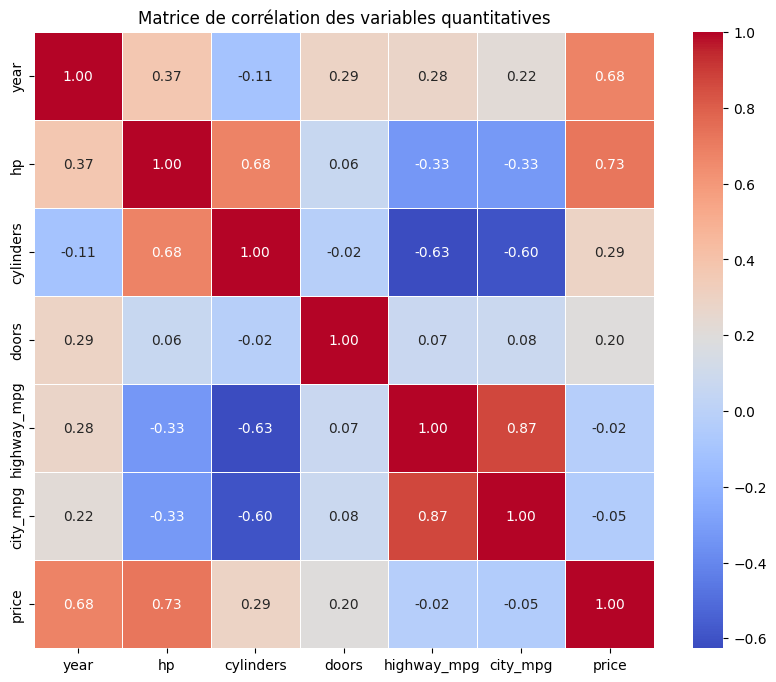
\includegraphics[width=1\textwidth]{correlation_matrix.png}
    \caption{Matrice de corrélation}
    \label{fig:correlation-matrix}
\end{figure}
\subsection{Champs utilisés pour le modèle}
Les champs suivants ont été utilisés pour le modèle : \textit{make, model, year, fuel\_type, hp, transmission, cylinders, drive, size, style}.


\section{Modèle et Entraînement}

\subsection{Algorithmes explorés}

Dans une démarche d'exploration comparative, trois approches ont été testées pour estimer le prix d’un véhicule à partir de ses caractéristiques techniques : \textbf{KNN}, \textbf{RNN} et \textbf{Random Forest}. Chacune de ces approches présente des avantages spécifiques :

\begin{itemize}
    \item \textbf{K-Nearest Neighbors (KNN)} : Bien que les données soient étiquetées, nous avons souhaité tester ce modèle car il permet de capturer des relations locales entre les caractéristiques des véhicules. Cependant, il peut être sensible à la dimensionnalité des données et nécessite une optimisation du paramètre \( k \). Pour cela, nous avons implémenté une recherche exhaustive similaire à une Grid Search, où nous avons testé chaque valeur de \( k \) dans une plage allant de 1 à 30. Cette approche nous a permis de déterminer la valeur optimale de \( k \) qui minimise l'erreur quadratique moyenne (RMSE).

    \item \textbf{Random Forest (RF)} : Ce modèle nous a semblé immédiatement pertinent en raison de sa capacité à gérer des données de grande dimension et à capturer des interactions complexes entre les variables. De plus, il est robuste face aux valeurs aberrantes et offre une bonne interprétabilité grâce à l'importance des variables.

    \item \textbf{Recurrent Neural Network (RNN)} : Les RNN sont particulièrement adaptés pour traiter des séquences de données, ce qui peut être intéressant si l'on considère l'historique des prix ou des caractéristiques temporelles. Cependant, leur entraînement peut être plus complexe et nécessite des ressources computationnelles importantes.
\end{itemize}



\subsection{Encodage}

\subsubsection{Target Encoding}

Pour les modèles KNN et RNN, nous avons opté pour le \textit{target encoding} sur la variable prix. Cette méthode s'est avérée la plus efficace pour ces algorithmes, car elle permet de transformer les variables catégorielles en valeurs numériques tout en préservant l'information sur la cible.

\subsubsection{Label Encoding}

Pour le modèle Random Forest (RF), nous avons utilisé le \textit{label encoding}, qui s'est révélé être le plus performant. Cette technique assigne une valeur numérique unique à chaque catégorie, ce qui est bien adapté aux arbres de décision qui composent la forêt aléatoire.

\subsection{Séparation des données et évaluation} 

Afin d’évaluer la performance de notre modèle sans le biaiser, nous avons choisi de diviser notre jeu de données en deux sous-ensembles : un ensemble d’entraînement et un ensemble de test. La proportion utilisée pour le test, définie par la variable \texttt{test\_size}, a été fixée à 30~\% des données. Cette séparation permet de mesurer la capacité du modèle à généraliser sur des données inédites, et ainsi de limiter le risque de surapprentissage (overfitting).


\subsection{Évaluation et Résultats}

\subsubsection{Validation croisée}

Nous avons utilisé la méthode de validation croisée K-Fold pour évaluer les performances des modèles. Cette approche permet de garantir une évaluation robuste en divisant les données en plusieurs sous-ensembles et en entraînant le modèle sur différentes combinaisons de ces sous-ensembles. Nous avons effectué une validation croisée avec 5 folds à chaque fois. Aucun des modèles n'a montré de disparité significative dans les résultats, ce qui indique qu'il n'y a pas d'overfitting. Cela aide à prévenir le surapprentissage et à assurer que le modèle ne
se contente pas de mémoriser les données d'entraînement, mais apprend plutôt à identifier
et à généraliser à partir de patterns sous-jacents.


\subsubsection{K-Nearest Neighbors (KNN)}

\begin{itemize}
    \item \textbf{Erreur quadratique moyenne (RMSE)} : \$3575.05
    \item \textbf{Erreur quadratique moyenne (RMSE) en pourcentage} : 12.28\%
    \item \textbf{Score \( R^2 \)} : 0.9463
\end{itemize}

\subsubsection{Random Forest (RF)}

\begin{itemize}
    \item \textbf{Erreur quadratique moyenne (RMSE)} : \$3237.02
    \item \textbf{Erreur quadratique moyenne (RMSE) en pourcentage} : 11.12\%
    \item \textbf{Score \( R^2 \)} : 0.9560
\end{itemize}

\subsubsection{Réseau de Neurones (RNN)}

\begin{itemize}
    \item \textbf{Erreur quadratique moyenne (RMSE)} : \$4055.24
    \item \textbf{Erreur quadratique moyenne (RMSE) en pourcentage} : 13.93\%
    \item \textbf{Score \( R^2 \)} : 0.9310
\end{itemize}

\subsection{Modèle choisi}

Nous avons opté pour le modèle \textbf{Random Forest (RF)} avec \textit{label encoding}. Cette décision repose sur plusieurs justifications :

\begin{itemize}
    \item \textbf{Performance supérieure} : Le modèle RF a démontré une meilleure performance en termes d'erreur quadratique moyenne (RMSE) et de score \( R^2 \) par rapport aux autres modèles testés.
    \item \textbf{Robustesse} : Les forêts aléatoires sont robustes face aux valeurs aberrantes et peuvent gérer efficacement les interactions complexes entre les variables.
    \item \textbf{Interprétabilité} : Le RF permet une meilleure interprétabilité des résultats grâce à l'importance des variables, ce qui est un atout pour comprendre les facteurs influençant le prix des véhicules.
\end{itemize}

Ces raisons combinées font du Random Forest le choix optimal pour notre projet.



\section{Interaction avec le Frontend}

\subsection{Variables saisies par l'utilisateur}

Nous avons cherché à rendre la saisie des données par l'utilisateur la moins contraignante possible. Pour ce faire, nous avons consulté plusieurs utilisateurs potentiels afin qu'ils nous communiquent les caractéristiques qu'ils jugent les plus importantes lors de l'achat d'une voiture. Les caractéristiques retenues sont les suivantes :
\begin{itemize}
    \item \textit{make} (marque)
    \item \textit{model} (modèle)
    \item \textit{year} (année)
    \item \textit{fuel\_type} (type de carburant)
    \item \textit{hp} (puissance en chevaux)
    \item \textit{transmission} (type de transmission)
\end{itemize}

Ces caractéristiques ont également été identifiées comme significatives dans nos analyses de corrélation, d'ANOVA et de Khi-deux. Nous les avons donc privilégiées dans l'interface utilisateur (UI). Cependant, pour ne pas compromettre les performances du modèle en négligeant les autres variables, nous avons procédé à l'inférence des variables manquantes.

\subsection{Inférence des variables manquantes}

Nous avons mis en place un système d'inférence pour estimer les valeurs des variables manquantes, telles que \textit{style}, \textit{drive}, \textit{cylinders} et \textit{size}. Ce système utilise des filtres successifs basés sur les caractéristiques saisies par l'utilisateur :
\begin{enumerate}
    \item Année du véhicule
    \item Puissance en chevaux (\textit{hp})
    \item Marque (\textit{make})
    \item Type de carburant (\textit{fuel\_type})
    \item Type de transmission (\textit{transmission})
\end{enumerate}

Pour les variables numériques, nous avons utilisé la moyenne des valeurs filtrées. Pour les variables catégorielles, nous avons retenu la catégorie la plus représentée après application des filtres. Si aucun élément n'est retourné par les filtres, la variable sera encodée avec la valeur \(-1\).


\subsection{Tolérance aux erreurs de saisie}

Pour gérer les cas où l'utilisateur fait des erreurs typographiques, comme écrire "5 series" au lieu de "serie 5" ou omettre un "s", nous avons mis en place un mécanisme de correspondance approximative. Ce mécanisme fonctionne comme suit :

\begin{enumerate}
    \item \textbf{Normalisation du texte} : Les entrées de l'utilisateur et les valeurs connues sont normalisées pour uniformiser leur format. Cela inclut la conversion en minuscules, la suppression des accents et des espaces superflus.
    \item \textbf{Recherche de correspondances approximatives} : Nous utilisons la bibliothèque \texttt{difflib} pour trouver des correspondances approximatives entre le texte normalisé de l'utilisateur et les valeurs connues. Si la similarité entre deux textes dépasse un seuil de 0.6, ils sont considérés comme correspondants.
    \item \textbf{Sélection de la meilleure correspondance} : Si une correspondance est trouvée, la valeur connue la plus proche est sélectionnée. Sinon, un message d'avertissement est affiché et la valeur est encodée comme \(-1\).
    \item \textbf{Encodage des valeurs} : Les valeurs saisies par l'utilisateur sont encodées en utilisant les encodeurs spécifiés. Si une valeur ne correspond pas exactement à une valeur connue, la correspondance approximative est utilisée.
    \item \textbf{Normalisation des valeurs numériques} : Les valeurs numériques sont normalisées en utilisant les valeurs minimales et maximales spécifiées dans les normalisateurs.
\end{enumerate}

\textbf{Inférence des données manquantes} :  
En plus de la correction des erreurs de saisie, nous avons intégré un mécanisme d'inférence pour compléter automatiquement certaines informations manquantes (notamment le nombre de cylindres, le type de transmission (\textit{drive}), la taille du véhicule (\textit{size}) et le style de carrosserie (\textit{style})).

Le processus d'inférence fonctionne comme suit :
\begin{enumerate}
    \item \textbf{Filtrage des données} : À partir des informations partiellement fournies par l'utilisateur (\textit{make}, \textit{year}, \textit{hp}, \textit{fuel\_type}, \textit{transmission}), nous filtrons la base de données interne pour trouver des véhicules similaires.
    \item \textbf{Approximation sur les catégories} : Pour les champs textuels tels que la marque ou le type de carburant, nous utilisons également une correspondance approximative afin de maximiser les chances de trouver des correspondances pertinentes.
    \item \textbf{Estimation des caractéristiques manquantes} : 
    \begin{itemize}
        \item Pour les variables numériques (par exemple, le nombre de cylindres), nous utilisons la moyenne des valeurs correspondantes trouvées dans la base de données (arrondie à l'entier le plus proche).
        \item Pour les variables catégorielles (par exemple, le type de transmission, la taille ou le style), nous utilisons la valeur la plus fréquente (\textit{mode}) parmi les correspondances trouvées.
    \end{itemize}
    \item \textbf{Valeurs par défaut} : En l'absence de correspondance suffisante (par exemple, aucun véhicule trouvé après filtrage), nous affectons des valeurs par défaut prudentes : \(4\) cylindres, transmission \textit{unknown}, taille \textit{unknown} et style \textit{unknown}.
\end{enumerate}

\textbf{Impact de l'inférence sur la prédiction} :  
Afin de vérifier que le mécanisme d'inférence n'altère pas significativement la performance du modèle de prédiction, nous avons réalisé une comparaison entre deux scénarios :
\begin{itemize}
    \item Prédiction du prix d'un véhicule en utilisant toutes les données complètes fournies manuellement par l'utilisateur.
    \item Prédiction du prix en utilisant seulement les données principales, complétées par le mécanisme d'inférence automatique.
\end{itemize}

Pour notre analyse, nous avons comparé plusieurs véhicules :
\begin{itemize}
    \item Ford Mustang 2020 (\textit{entrée manuelle partielle, modèle différent dans le dataset}),
    \item Kia Sportage 2017 (\textit{entrée correspondante au dataset}),
    \item Audi 100 1993 (\textit{entrée correspondante au dataset}),
    \item BMW 5 Series 2016 (\textit{entrée correspondante au dataset}).
\end{itemize}

Les résultats obtenus sont les suivants :

\begin{center}
\begin{tabular}{|c|c|c|}
\hline
\textbf{Véhicule} & \textbf{Prix (données complètes)} & \textbf{Prix (avec inférence)} \\
\hline
Ford Mustang & \$55,944.82 & \$64,681.57 \\
Kia Sportage & \$24,972.60 & \$26,400.51 \\
Audi 100 & \$2,015.20 & \$2,039.68 \\
BMW 5 Series & \$51,219.85 & \$44,736.67 \\
\hline
\textbf{Moyenne} & \$33,538.12 & \$34,464.61 \\
\hline
\end{tabular}
\end{center}

On observe une différence de \$926.49 entre les deux moyennes, soit un écart relatif de \textbf{2.76\%}. Ce faible écart confirme que le mécanisme d'inférence maintient une bonne qualité de prédiction globale, malgré des données initiales partielles. 

\textbf{Discussion} :  
La légère surévaluation de la Ford Mustang s'explique par le fait que le modèle utilisé ne correspond pas exactement à celui présent dans le dataset (modèle de génération différente), ce qui ne permet pas de savoir le prix exacte dans la réalité. En revanche, les trois autres véhicules correspondent précisément à des enregistrements existants dans la base, ou à des variantes très proches, ce qui justifie l'excellent alignement des prédictions.

Cet écart reste acceptable dans le cadre de notre application, car :
\begin{itemize}
    \item La prédiction du prix automobile est naturellement sujette à des variations de l'ordre de 10 à 20\% dans l'industrie, même entre véhicules similaires.
    \item Le mécanisme d'inférence utilise uniquement des valeurs réalistes extraites du dataset, en évitant toute création artificielle d'information.
    \item L'objectif principal est de minimiser la saisie utilisateur tout en offrant une estimation de qualité raisonnable.
\end{itemize}

Nous considérons que ce niveau d'écart est satisfaisant pour un projet académique. Toutefois, un peaufinage plus approfondi des filtres de sélection (par exemple, en affinant la recherche selon la puissance exacte ou en prenant en compte davantage de variables contextuelles comme le style précis) pourrait permettre de réduire encore cet écart à l'avenir.


\textbf{Justification du choix de l'inférence} :  
L'objectif est de minimiser l'effort de saisie demandé à l'utilisateur en déduisant automatiquement des informations prévisibles à partir des données déjà fournies. Les variables comme \textit{cylinders}, \textit{drive}, \textit{size} et \textit{style} sont généralement directement associées à un véhicule et peuvent être prédictibles à partir de ses caractéristiques principales (marque, puissance, carburant, transmission, etc.).  
En revanche, nous n'avons pas tenté d'inférer des informations comme le \textit{model}, car cette variable est beaucoup plus spécifique et créative : il n'est pas réaliste d'essayer d'inventer ou de prédire un nom de modèle automobile. Le modèle est une donnée d'identification précise qu'il est indispensable que l'utilisateur fournisse explicitement.  
Afin d'appuyer cette approche, nous avons également réalisé un sondage auprès d'un panel d'utilisateurs pour identifier les variables qu'ils seraient prêts à renseigner en priorité. Ce sondage a confirmé que des éléments tels que la marque, l'année, la motorisation et la transmission sont perçus comme simples et naturels à renseigner, tandis que des variables plus techniques comme le nombre de cylindres, la taille du véhicule ou son style sont moins spontanément connues et devraient donc être inférées automatiquement pour améliorer l'expérience utilisateur.

\subsection{Affichage des résultats}

Les résultats sont affichés dans le frontend sous cette forme : 

\begin{figure}[H]
    \centering
    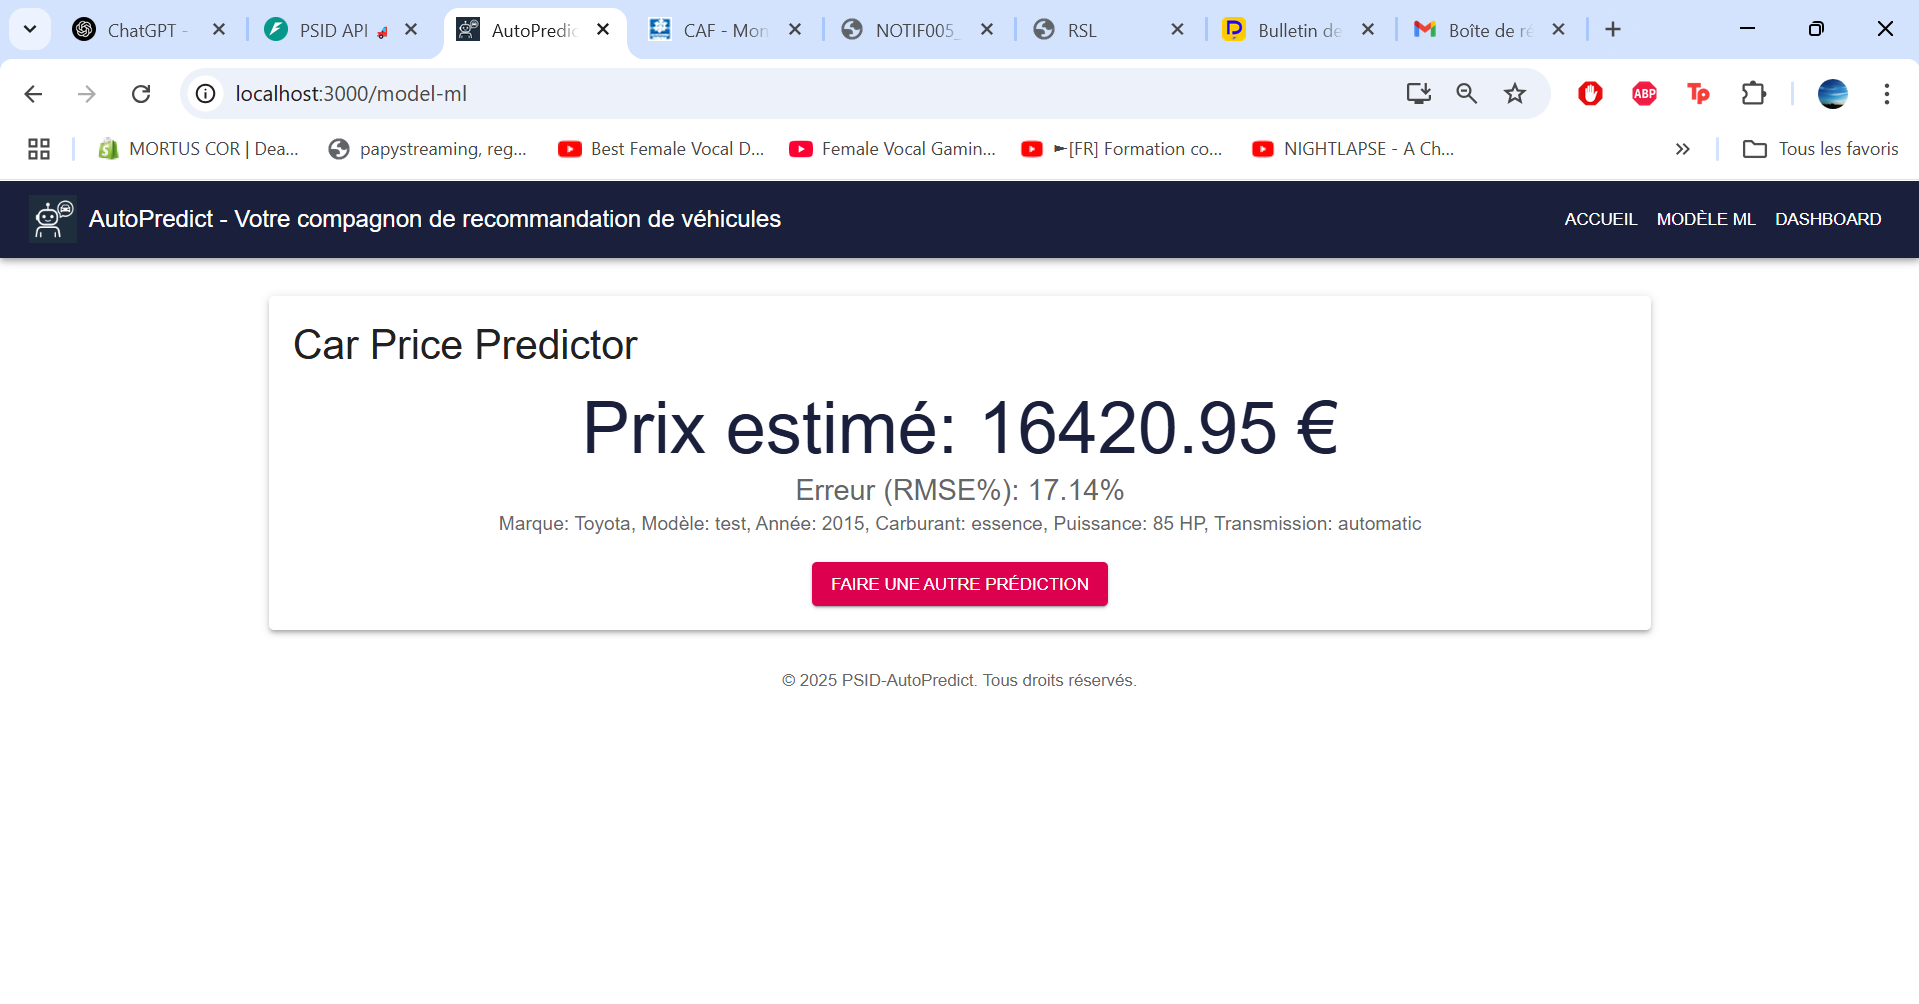
\includegraphics[width=1\textwidth]{resultats.png}
    \caption{Affichage des résultats}
    \label{fig:resultats}
\end{figure}
Le prix estimé est affiché en dollars puisqu'il s'agit d'un dataset américain. Nous avons également affiché le taux RMSE en pourcentage pour donner une idée de la précision du modèle. Ainsi que les données envoyées à l'API pour que l'utilisateur puisse vérifier les données qu'il a saisies.

\end{document}
